\section{Phương pháp thực hiện}

\subsection{Mục tiêu thực nghiệm}

Pipeline thực nghiệm được xây dựng để kiểm tra đồng thời hai lớp vấn đề. Lớp thứ nhất là chất lượng phân loại giữa benign traffic và DDoS traffic. Lớp thứ hai là hiệu quả giảm thiểu khi đưa quyết định pushback vào chuỗi xử lý. Vì vậy, phương pháp của nhóm không chỉ dừng ở bước huấn luyện mô hình mà còn bao gồm cả phần mô phỏng phản ứng của mạng sau khi có kết quả phân loại.

\subsection{Dữ liệu và đặc trưng}

Nguồn dữ liệu chính của project là tập \texttt{combine.csv} được trích từ CICIDS2017 và chuẩn hóa về bài toán nhị phân: \texttt{BENIGN} và nhóm Wednesday DoS. Trong reproduction chính, hệ thống ưu tiên một số feature có liên hệ trực tiếp tới khả năng biểu diễn trong data plane, chẳng hạn \texttt{protocol}, \texttt{init\_win\_bytes\_forward}, \texttt{fwd\_header\_length}, \texttt{packet\_length\_mean} và \texttt{flow\_packets\_persecond}. Dữ liệu sau đó được ép kiểu số, xử lý \texttt{NaN}/\texttt{inf}, cắt bớt ngoại lai và chia train/test theo tỉ lệ 80/20.

\subsection{Ba mô hình được so sánh}

Ba mô hình được dùng trong toàn bộ thực nghiệm gồm:
\begin{enumerate}
\item \textbf{Decision Tree (DT):} baseline đơn giản, dễ hiểu, dễ chuyển thành các điều kiện dạng ``feature $\le$ threshold''.
\item \textbf{Random Forest (RF):} thường đạt chất lượng tốt nhưng số threshold lớn, do đó khó phù hợp với data plane.
\item \textbf{DT-CTS:} mô hình trọng tâm của project, giới hạn số threshold trên mỗi feature để giảm độ phức tạp triển khai.
\end{enumerate}

Ngoài accuracy, precision, recall và F1, project còn đo \textit{threshold count}. Chỉ số này không thay thế hoàn toàn các tài nguyên phần cứng như TCAM hay SRAM, nhưng là một đại diện hợp lý để so sánh footprint giữa các mô hình trong môi trường tái hiện phần mềm.

\subsection{Cơ chế hierarchical confidence-aware pushback}

Cải tiến chính của báo cáo nằm ở policy giảm thiểu mới. Thay vì block source ngay khi có một dự đoán attack, cơ chế này gán cho mỗi source một \textit{suspicion score}. Điểm số này tăng lên dựa trên các bằng chứng sau:
\begin{itemize}
\item edge detector dự đoán malicious,
\item core detector dự đoán malicious,
\item edge và core cùng đồng thuận,
\item traffic có dấu hiệu spike bất thường.
\end{itemize}

Song song với đó, suspicion score cũng giảm dần theo thời gian nếu source không tiếp tục có hành vi đáng nghi. Cách làm này giúp hệ thống không giữ trạng thái cảnh báo quá lâu chỉ vì một burst ngắn hạn.

Từ score hiện tại, hệ thống chọn một trong bốn mức phản ứng:
\begin{enumerate}
\item \texttt{monitor},
\item \texttt{local rate-limit},
\item \texttt{upstream pushback},
\item \texttt{hard block}.
\end{enumerate}

Mức phản ứng càng cao thì tỷ lệ traffic còn được forward tới victim càng thấp. Nói cách khác, pushback ở đây không còn là một quyết định nhị phân nữa, mà trở thành một quá trình leo thang có kiểm soát.

\begin{table}
\caption{Các thành phần chính của suspicion score và mức phản ứng trong policy mới.}
\label{tab:score-policy}
\centering
\begin{tabular}{p{3.0cm}p{2.2cm}p{4.6cm}}
\toprule
\textbf{Thành phần} & \textbf{Giá trị} & \textbf{Ý nghĩa} \\
\midrule
Edge evidence & +2 & Tín hiệu nghi ngờ sớm từ edge detector \\
Core evidence & +4 & Xác nhận mạnh hơn từ core detector \\
Agreement bonus & +3 & Tăng độ tin cậy khi edge và core cùng dự đoán attack \\
Spike evidence & +2 & Bổ sung bằng chứng khi traffic tăng đột biến \\
Decay & -1 / window & Giảm cảnh báo nếu source không tiếp tục đáng nghi \\
Monitor & score $\geq 3$ & Theo dõi, chưa cắt traffic \\
Local rate-limit & score $\geq 6$ & Giảm một phần traffic ở cục bộ \\
Upstream pushback & score $\geq 12$ & Đẩy hành động lọc về switch phía trước \\
Hard block & score $\geq 24$ + core=attack & Chặn hoàn toàn source khi bằng chứng đủ mạnh \\
\bottomrule
\end{tabular}
\end{table}

\subsection{Mô hình hệ thống và pipeline thực nghiệm}

\begin{figure}
\centering
\fbox{
\begin{minipage}{0.88\textwidth}
\vspace{0.2cm}
\centering
\textbf{Dataset CICIDS2017 subset}

$\Downarrow$

\textbf{Tiền xử lý và chọn feature}

$\Downarrow$

\textbf{Huấn luyện DT / RF / DT-CTS}

$\Downarrow$

\textbf{Đánh giá classification + threshold efficiency}

$\Downarrow$

\textbf{Sinh pushback trace theo source và time window}

$\Downarrow$

\textbf{Edge DT-CTS + Core DT-CTS + Spike signal}

$\Downarrow$

\textbf{Suspicion score}

$\Downarrow$

\textbf{Monitor $\rightarrow$ Local rate-limit $\rightarrow$ Upstream pushback $\rightarrow$ Hard block}
\vspace{0.2cm}
\end{minipage}
}
\caption{Pipeline thực nghiệm của project, từ phân loại tới mô phỏng giảm thiểu.}
\label{fig:pipeline}
\end{figure}

Hình~\ref{fig:pipeline} cho thấy logic tổng thể của hệ thống. Khác với cách trình bày thuần lý thuyết của bài báo gốc, pipeline trong project được tổ chức để có thể chạy lại hoàn toàn bằng mã nguồn Python, nhưng vẫn giữ đúng tinh thần ``phát hiện nhẹ, phản ứng sớm, giảm thiểu theo mức'' của SISTAR.

\begin{figure}
\centering
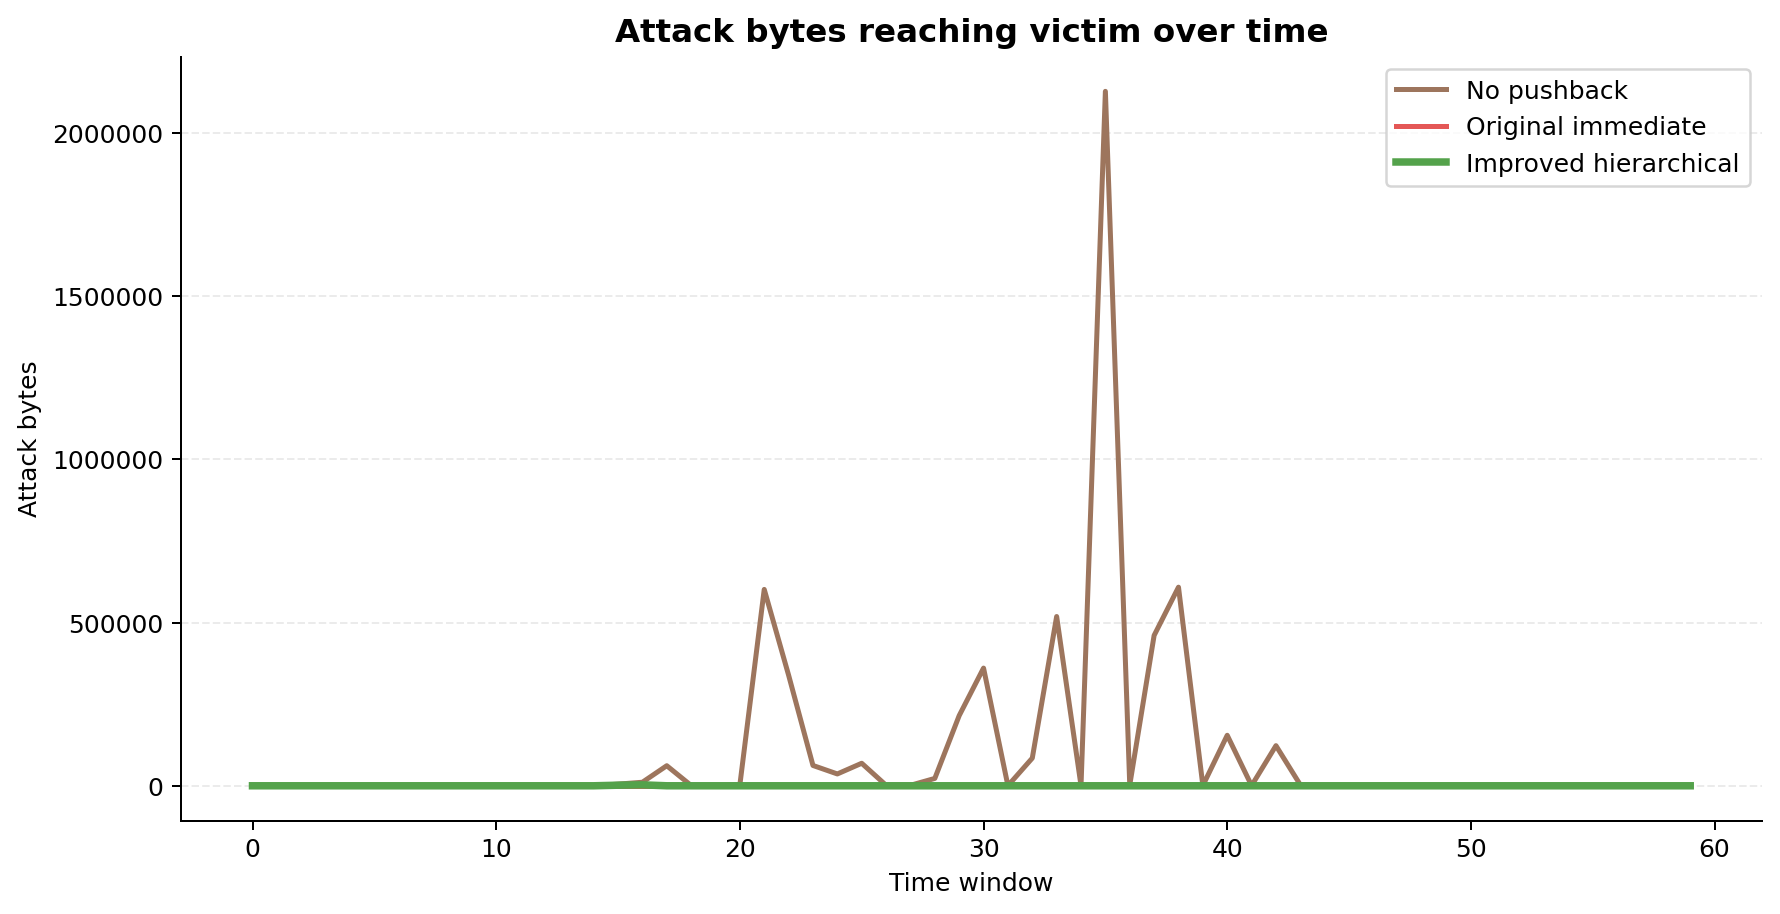
\includegraphics[width=0.9\textwidth]{figures/attack_timeline.png}
\caption{Diễn biến attack bytes tới victim theo thời gian giữa ba policy. Đường cong của hierarchical pushback bám sát immediate pushback về hiệu quả cắt attack, nhưng đạt được điều đó bằng cơ chế leo thang mềm hơn.}
\label{fig:attack-timeline}
\end{figure}
